\begin{figure}%[b]
    	\centering
    	\begin{minipage}{1\textwidth}
    		\begin{minipage}{.6\textwidth}
    			\centering
    			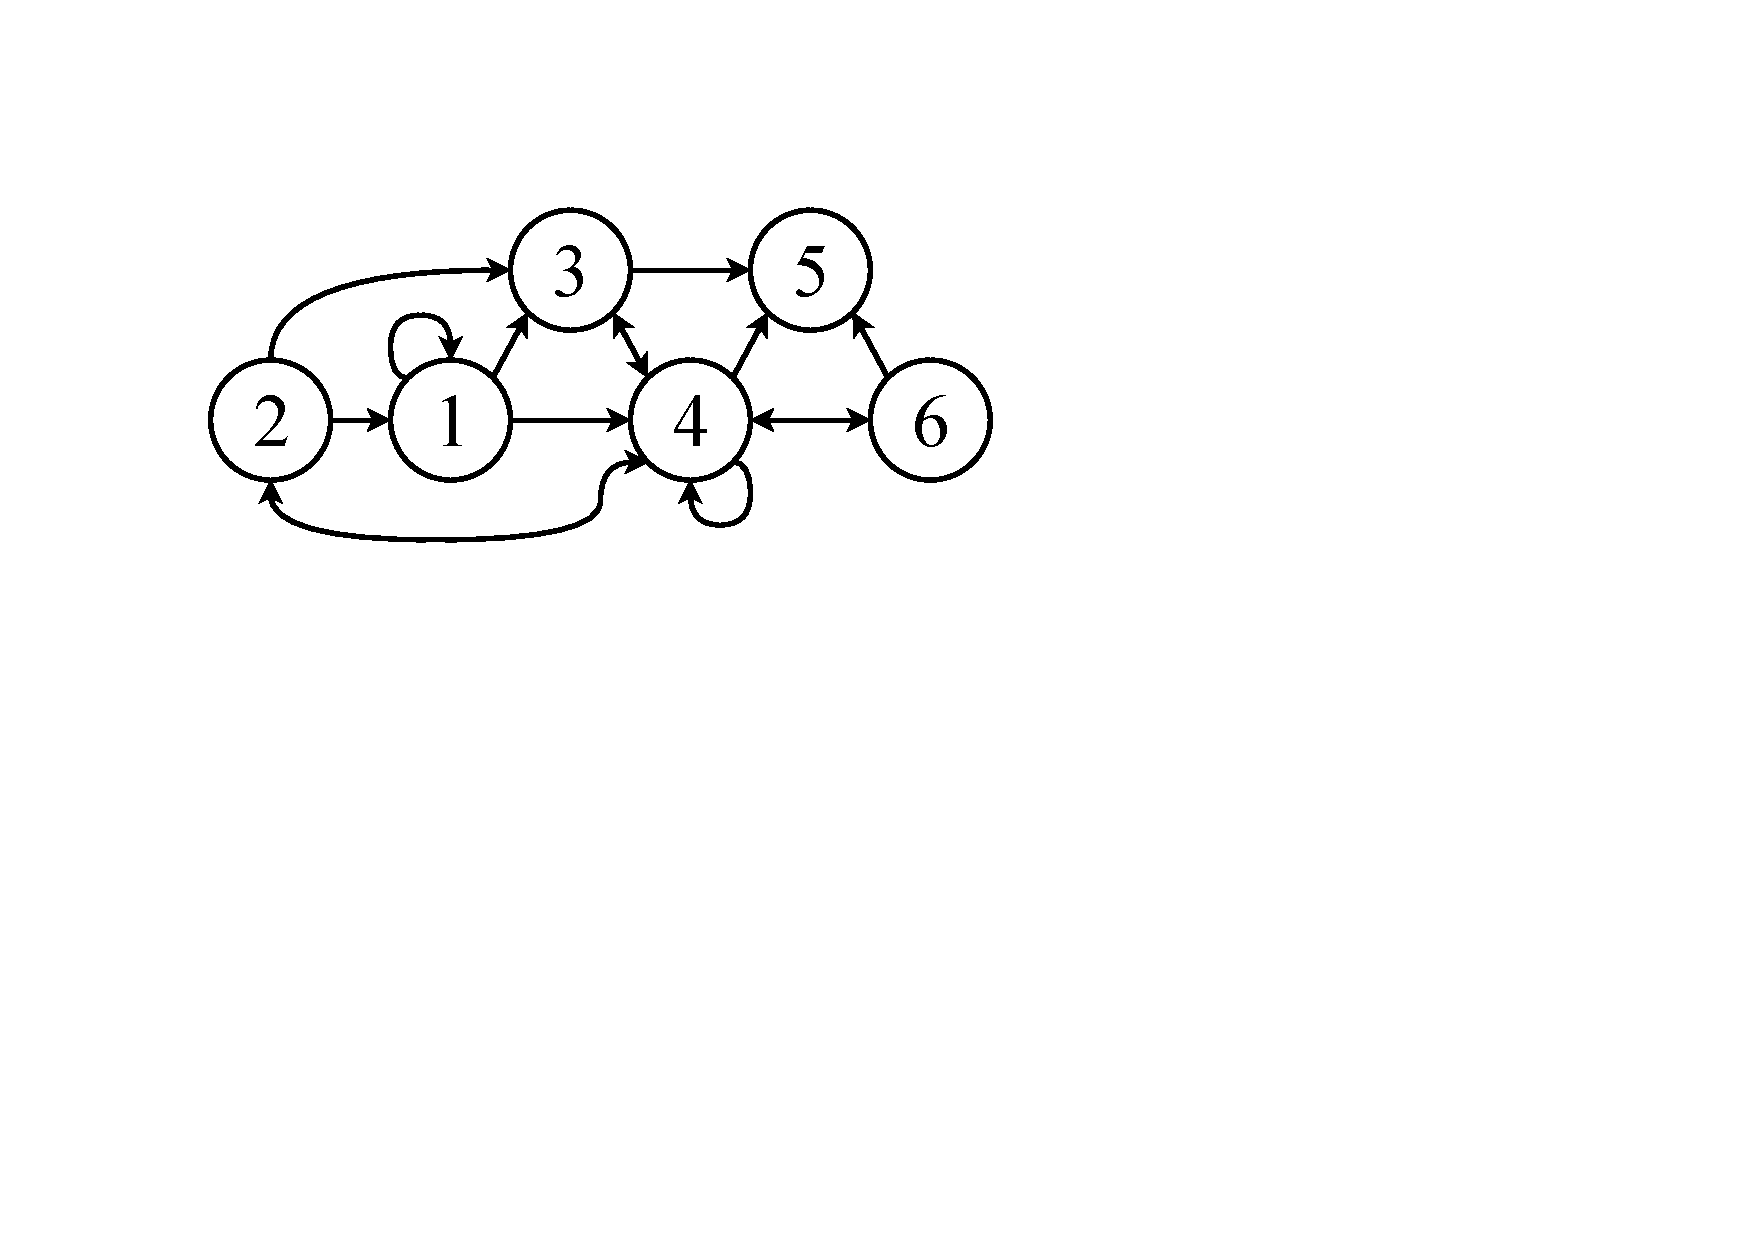
\includegraphics[scale=.3, clip,  trim=90 330 350 90]{img/arte/graphs-repair.pdf}
    		
    			(a)
    		\end{minipage}
    		\begin{minipage}{.35\textwidth}
    			\centering
    			\vspace{5mm}
		    	\begin{tabular}{|l|l|}
		    		\hline
		    		B1 & 111101 \\
		    		\hline
		    		B2 & 1111001\\
		    		\hline
		    	\end{tabular}
		    	\vspace{5mm}
		    	
    			(c)
    		\end{minipage}
    	\end{minipage}
    	\vspace{5mm}
    	
    	\begin{minipage}{1\textwidth}
    		\centering

		\begin{tabular}{l||l|l|l|l|l|l|l|l|l|l|l|l|l|l|l|l|l|l|l|l|l|}
			\toprule
			$T(G)$ & -1 & 1 & 3 & 4 & -2 & 1 & 3 & 4 & -3 & 4 & 5 & -4 & 3 & 4 & 5 & 6 & -5 & -6 & 4 & 5 \\
			\midrule
			$7 \rightarrow 4 \; 5$ & -1 & 1 & 3 & 4 & -2 & 1 & 3 & 4 & -3 & 7 & -4 & 3 & 7 & 6 & -5 & -6 & 7 \\
			\cline{1-18}
			$8 \rightarrow 1 \; 3$ & -1 & 8 & 4 & -2 & 8 & 4 & -3 & 7 & -4 & 3 & 7 & 6 & -5 & -6 & 7 \\
			\cline{1-16}
			$9 \rightarrow 8 \; 4$ & -1 & 9 & -2 & 9 & -3 & 7 & -4 & 3 & 7 & 6 & -5 & -6 & 7 \\
			\cline{1-14}
			Borrar $<0$ & 9 & 9 & 7 & 3 & 7 & 6 & 7 \\
			\cline{1-8}
		\end{tabular}				
		\vspace{5mm}
		
		(b)
    	\end{minipage}

    \caption{Ejemplo para Re-Pair aplicado a grafos por Claude y Navarro. (a) Grafo de ejemplo. (b) Listado concatenado $T(G)$ y resultado final luego de tres reemplazos y eliminar nodos de referencia. (c) Bitmaps indicadores de nodos de referencia removidos.}
    \label{fig:repairCN}
\end{figure}
